\documentclass[12pt]{article}

% Set the page to be letter paper and have small margins
\usepackage{geometry}
\geometry{letterpaper, left=15mm, right=15mm, top=15mm, bottom=20mm}


% LuaLaTeX font setup
\usepackage{fontspec}
\usepackage{unicode-math}

% Text font
\setmainfont{DejaVu Serif}

% Math font
\setmathfont{STIX Two Math}

% Optional: fake bold math (Fira Math has no bold)
\usepackage{xfakebold}

\usepackage{parskip}
\usepackage{amsmath}
\usepackage{amsthm}
\usepackage{enumitem}
\usepackage{multicol}
\usepackage{graphicx}
\usepackage{pgfplots}
\pgfplotsset{compat=1.18}
\usepackage{cancel}

\begin{document}

\noindent
Jeffrey Morris
\hfill
MATH 4306-010
\newline
January 19, 2026

\begin{center}
    \Large{Homework 1}
\end{center}

\begin{enumerate}[label=\textbf{\arabic*}.]
    %
    % Problem 1
    %
    \item Find the Fourier coefficients of the functions given in what follows. All are supposed to be periodic with period $2\pi$. Sketch the graph of the function.
          \begin{enumerate}[label=\textbf{\alph*}.]
              % Increase counter to make the element be (b)
              \addtocounter{enumii}{1}
              %
              % Problem 1-b
              %
              \item $f(x)=\left|x\right|,\qquad -\pi<x<\pi$
                    \begin{align*}
                        a_0= & \frac{1}{2\pi}\int_{-\pi}^{\pi}f(x)\,dx           \\
                        a_0= & \frac{1}{\pi}\int_{0}^{\pi}f(x)\,dx               \\
                        a_0= & \frac{1}{\pi}\int_{0}^{\pi}x\,dx                  \\
                        a_0= & \frac{1}{\pi}\left[\frac{x^2}{2}\right]_{0}^{\pi} \\
                        a_0= & \frac{1}{\pi}\cdot\frac{\pi^2}{2}                 \\
                        a_0= & \boxed{\frac{\pi}{2}}
                    \end{align*}
                    \begin{align*}
                        a_n= & \frac{1}{\pi}\int_{-\pi}^{\pi}f(x)\cos(nx)\,dx                                                                            \\
                        a_n= & \frac{2}{\pi}\int_{0}^{\pi}f(x)\cos(nx)\,dx                                                                               \\
                        a_n= & \frac{2}{\pi}\int_{0}^{\pi}x\cos(nx)\,dx                                                                                  \\
                        a_n= & \frac{2}{\pi}\left[\left.\frac{x\sin(nx)}{n}\right|_{0}^{\pi}-\int_{0}^{\pi}\frac{\sin(nx)}{n}\,dx\right]                 \\
                        a_n= & \frac{2}{\pi}\left[\left(\frac{\pi\cancelto{0}{\sin(nx)}}{n}-0\right)-\left.\frac{-\cos(nx)}{n^2}\right|_{0}^{\pi}\right] \\
                        a_n= & \frac{2}{\pi}\left(\frac{\cos(n\pi)}{n^2}-\frac{\cancelto{1}{\cos(0)}}{n^2}\right)                                        \\
                        a_n= & \frac{2}{\pi}\left(\frac{(-1)^n}{n^2}-\frac{1}{n^2}\right)                                                                \\
                        a_n= &
                        \boxed{
                            \begin{cases}
                                0,                 & \text{if } n \text{ is even} \\
                                \frac{-4}{n^2\pi}, & \text{if } n \text{ is odd}
                            \end{cases}
                        }
                    \end{align*}
                    \newpage
                    \begin{gather*}
                        b_n=\frac{1}{\pi}\int_{-\pi}^{\pi}f(x)\sin(nx)\,dx \\
                        \text{Because $f(x)$ is odd, $b_n=\boxed{0}$}
                    \end{gather*}
                    \begin{center}
                        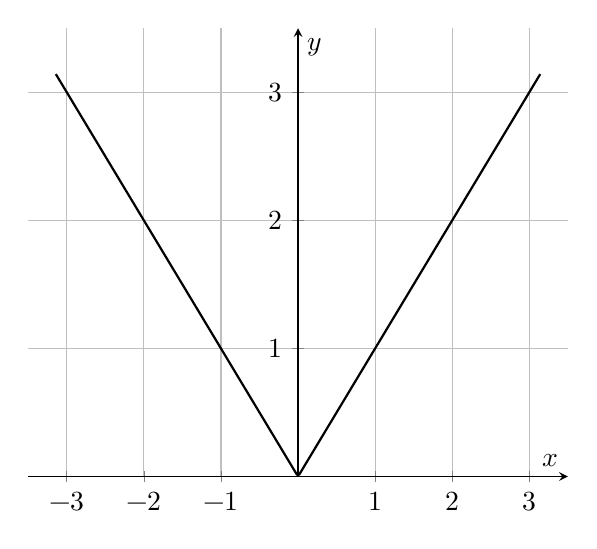
\begin{tikzpicture}
                            \begin{axis}[
                                    axis lines=middle,
                                    grid=both,
                                    xmin=-3.5, xmax=3.5,
                                    ymin=0, ymax=3.5,
                                    xlabel={$x$}, ylabel={$y$},
                                    samples=200,
                                    domain=-pi:pi,
                                ]
                                \addplot[thick]{abs(x)};
                            \end{axis}
                        \end{tikzpicture}
                    \end{center}
                    % Increase counter to make the element be (d)
                    \addtocounter{enumii}{1}
                    %
                    % Problem 1-d
                    %
              \item $f(x)=\left|\sin(x)\right|$
                    \begin{align*}
                        f(-x) & =\left|\sin(-x)\right|            \\
                              & =\left|-\sin(x)\right|            \\
                              & =\left|sin(x)\right| = f(x)       \\
                              & \Rightarrow f(x) \text{ is even.}
                    \end{align*}
                    \begin{align*}
                        a_0= & \frac{1}{2\pi}\int_{-\pi}^{\pi}f(x)\,dx      \\
                        a_0= & \frac{1}{\pi}\int_{0}^{\pi}\sin(x)\,dx       \\
                        a_0= & \frac{1}{\pi}\left[-\cos(x)\right]_{0}^{\pi} \\
                        a_0= & \frac{1}{\pi}\left[-\cos(\pi)+\cos(0)\right] \\
                        a_0= & \frac{1}{\pi}\cdot 2                         \\
                        a_0= & \boxed{\frac{2}{\pi}}
                    \end{align*}
                    \begin{align*}
                        a_n= & \frac{1}{\pi}\int_{-\pi}^{\pi}f(x)\cos(nx)\,dx                                                                                                                                     \\
                        a_n= & \frac{2}{\pi}\int_{0}^{\pi}\sin(x)\cos(nx)\,dx                                                                                                                                     \\
                        a_n= & \frac{2}{\pi}\int_{0}^{\pi}\frac{1}{2}\left[\sin(x+nx)+sin(x-nx)\right]\,dx                                                                                                        \\
                        a_n= & \frac{1}{\pi}\sin\left((n+1)\cdot x\right)-\sin\left((n-1)\cdot x\right)\,dx                                                                                                       \\
                        a_n= & \frac{1}{\pi} \left[ \frac{-\cos\left((n+1) \cdot x\right)}{n+1} + \frac{\cos\left((n-1)\cdot x\right)}{n-1} \right]_{0}^{\pi}                                                     \\
                        a_n= & \frac{1}{\pi} \left[ \left( \frac{-\cos\left((n+1) \cdot \pi\right)}{n+1} + \frac{\cos\left((n-1)\cdot\pi\right)}{n-1}\right) - \left(\frac{-1}{n+1} + \frac{1}{n+1}\right)\right] \\
                        a_n= & \frac{1}{\pi} \left[ \frac{(-1)^n}{n+1} + \frac{-(-1)^n}{n-1} + \frac{1}{n+1} + \frac{-1}{n-1}\right]                                                                              \\
                        a_n= & \frac{1}{\pi} \left[ \frac{1+(-1)^n}{n+1} - \frac{1+(-1)^n}{n-1} \right]                                                                                                           \\
                        a_n= & \frac{1+(-1)^n}{\pi} \left[ \frac{-2}{n^2-1} \right]                                                                                                                               \\
                        a_n= &
                        \boxed{
                            \begin{cases}
                                0,                                          & \text{if $n$ is odd}  \\
                                \frac{-4}{\left( n^2 - 1 \right)\cdot \pi}, & \text{if $n$ is even}
                            \end{cases}
                        }
                    \end{align*}
                    \begin{gather*}
                        b_n=\frac{1}{\pi}\int_{-\pi}^{\pi}f(x)\sin(nx)\,dx \\
                        \text{Since $f(x)$ is even, $b_n=\boxed{0}$ }
                    \end{gather*}
                    \begin{center}
                        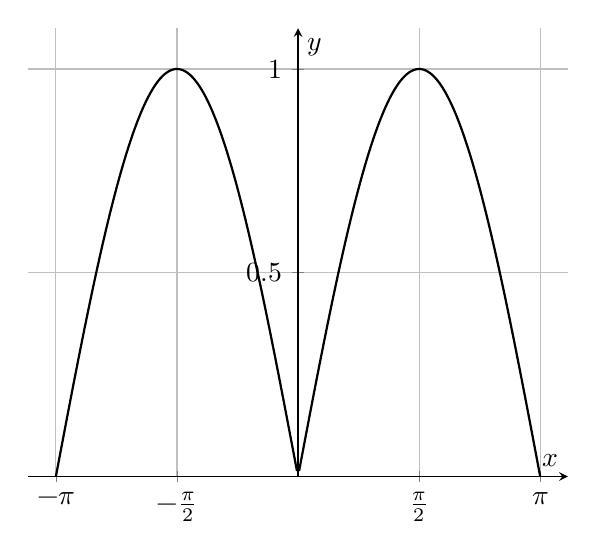
\begin{tikzpicture}
                            \begin{axis}[
                                    axis lines=middle,
                                    grid=both,
                                    xmin=-3.5, xmax=3.5,
                                    ymin=0, ymax=1.1,
                                    xtick={-pi,-pi/2,0,pi/2,pi},
                                    xticklabels={$-\pi$,$-\frac{\pi}{2}$,$0$,$\frac{\pi}{2}$,$\pi$},
                                    ytick={0, 0.5, 1},
                                    xlabel={$x$}, ylabel={$y$},
                                    samples=200,
                                    domain=-pi:pi,
                                ]
                                \addplot[thick]{abs(sin(deg(x)))};
                            \end{axis}
                        \end{tikzpicture}
                    \end{center}
          \end{enumerate}
          %
          % Problem 2
          %
          \newpage
    \item Find the Fourier series of each of the following functions. Sketch the graph of the periodic extension of $f$ for at least two periods.
          \begin{enumerate}[label=\textbf{\alph*}.]
              % Set the counter to (b)
              \addtocounter{enumii}{1}
              %
              % Problem 2-b
              %
              \item
                    $  f(x) =
                        \begin{cases}
                            -1, & -2 < x < 0 \\
                            1,  & 0 < x < 2
                        \end{cases}
                    $
                    \begin{gather*}
                        f(-x)=-f(x) \Rightarrow f(x) \text{ is odd.} \\
                        \text{Since $f(x)$ is odd: $a_0 = \boxed{0}$ and $a_n=\boxed{0}$}
                    \end{gather*}
                    \begin{align*}
                        b_n & =\frac{1}{L}\int_{-L}^{L}f(x)\sin\left(\frac{n\pi x}{L}\right)\,dx   \\
                        b_n & =\frac{1}{2}\int_{-2}^{2}f(x)\sin\left( \frac{n\pi x}{2} \right)\,dx \\
                        b_n & =1\int_{0}^{2}1\cdot\sin\left( \frac{n\pi x}{2} \right)\,dx          \\
                        b_n & =\frac{2}{n\pi}\left.\cos\left( \frac{n\pi x}{2} \right)\right|_0^2  \\
                        b_n & =\frac{-2}{n\pi}\left( \cos(n\pi) -\cos(0) \right)                   \\
                        b_n & =\frac{-2}{n\pi}\left( (-1)^n -1 \right)                             \\
                        b_n & =
                        \boxed{
                            \begin{cases}
                                0,              & \text{if $n$ is even} \\
                                \frac{4}{n\pi}, & \text{if $n$ is odd}
                            \end{cases}
                        }
                    \end{align*}
                    \begin{align*}
                        f(x) & =a_0+\sum_{n=1}^{\infty}\left( a_n \cos\left( \frac{n\pi x}{L} \right) + b_n\sin\left( \frac{n\pi x}{L} \right) \right) \\
                        f(x) & =\boxed{\sum_{n=\text{odd}}^{\infty}\left( \frac{4}{n\pi}\sin \left( \frac{n\pi x}{2} \right)\right)}
                    \end{align*}
                    \begin{center}
                        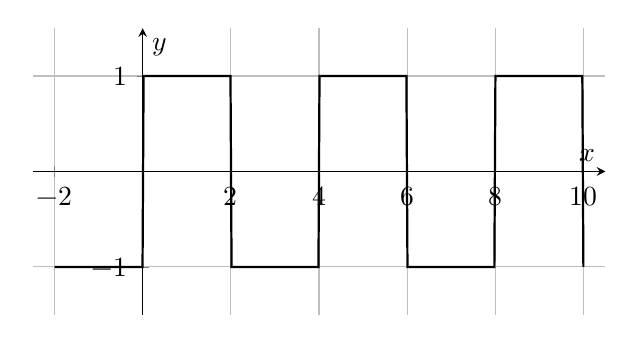
\begin{tikzpicture}
                            \begin{axis}[
                                    axis lines=middle,
                                    grid=both,
                                    scale only axis=true,
                                    width=.6\textwidth,
                                    height=0.3\textwidth,
                                    xmin=-2.5, xmax=10.5,
                                    ymin=-1.5, ymax=1.5,
                                    xlabel={$x$}, ylabel={$y$},
                                    samples=500,
                                    domain=-2:10,
                                ]
                                \addplot[thick]{
                                    (mod(x+2,4)-2 < 0)*(-1)
                                    + (mod(x+2,4)-2 > 0)*( 1)
                                };
                            \end{axis}
                        \end{tikzpicture}
                    \end{center}
          \end{enumerate}
          %
          % Problem 3
          %
          \newpage
    \item Identify each of the following as being even, odd, or neither.
          \begin{enumerate}[label=\textbf{\alph*}.]
              %
              % Problem 3-a
              %
              \item $f(x)=x$
                    \begin{align*}
                        f(-x) & =-x                               \\
                        -f(x) & =-x \Rightarrow\boxed{\text{odd}}
                    \end{align*}
                    %
                    % Problem 3-b
                    %
              \item $f(x)=\left|x\right|$
                    \begin{align*}
                        f(-x) & =|-x|                                 \\
                              & =|x|                                  \\
                        f(x)  & = |x| \Rightarrow \boxed{\text{even}}
                    \end{align*}
                    %
                    % Problem 3-c
                    %
              \item $f(x)=\left|\cos(x)\right|$
                    \begin{align*}
                        f(-x) & =|\cos(-x)|                             \\
                              & =|\cos(x)|                              \\
                        f(x)  & =|\cos(x)\Rightarrow\boxed{\text{even}}
                    \end{align*}
                    %
                    % Problem 3-d
                    %
              \item $f(x)=\arcsin(x)$
                    \begin{align*}
                        f(-x) & =\arcsin(-x)                                \\
                              & =-\arcsin(x)                                \\
                        -f(x) & =-\arcsin(x) \Rightarrow \boxed{\text{odd}}
                    \end{align*}
                    %
                    % Problem 3-e
                    %
              \item $f(x)=x\cos(x)$
                    \begin{align*}
                        f(-x) & =-x\cos(-x)                             \\
                              & =-x\cos(x)                              \\
                        -f(x) & =-x\cos(x)\Rightarrow\boxed{\text{odd}}
                    \end{align*}
                    %
                    % Problem 3-f
                    %
              \item $f(x)=x+\cos(x+1)$
                    \begin{align*}
                        f(-x) & =-x+\cos(-x+1)                    \\
                        -f(x) & =-x-\cos(x+1)                     \\
                        f(x)  & =x+\cos(x+1)                      \\
                              & \Rightarrow\boxed{\text{neither}}
                    \end{align*}
          \end{enumerate}
          %
          % Problem 4
          %
    \item Justify or prove these statements:
          \begin{enumerate}[label=\textbf{\alph*}.]
              %
              % Problem 4-a
              %
              \item If $h(x)$ is an odd function, then $\left|h(x)\right|$ is an even function.
                    \begin{align*}
                        \text{Since } h(-x) & =-h(x)                                \\
                        \text{And }|-x|     & =|x|                                  \\
                        \text{Then }|h(x)|  & =|-h(x)|                              \\
                        |-h(x)|             & = |h(-x)|                             \\
                                            & \therefore\; |h(x)| \text{ is even. }
                    \end{align*}
                    %
                    % Problem 4-b
                    %
              \item If $f(x)$ is defined for all positive $x$, then $f(\left|x\right|)$ is an even function.
                    \begin{align*}
                        \text{Since }f(|-x|) & =f(|x|)                             \\
                        \text{Then } f(-x)   & = f(x)                              \\
                                             & \therefore\; f(|x|) \text{ is even}
                    \end{align*}
                    %
                    % Problem 4-c
                    %
              \item If $f(x)$ is defined for all $x$ and $g(x)$ is any even function, then $f\left(g(x)\right)$ is even.
                    \begin{align*}
                        \text{Since } g(x)   & =g(-x)                               \\
                        \text{Then } f(g(x)) & = f(g(-x))                           \\
                                             & \therefore\; f(g(x)) \text{ is even}
                    \end{align*}
                    %
                    % Problem 4-d
                    %
              \item If $h(x)$ is an odd function, $g(x)$ is even, and $g(x)$ is defined for all $x$, then $g\left(h(x)\right)$ is an even function.
                    \begin{align*}
                        \text{Since } h(-x)   & =-h(x)                               \\
                        \text{And } g(x)      & =g(-x)                               \\
                        \text{Then } g(h(-x)) & = g(-h(x))                           \\
                        g(h(-x))              & = g(h(x))                            \\
                                              & \therefore\; g(h(x)) \text{ is even}
                    \end{align*}
          \end{enumerate}
    \item Find the Fourier series of the function $f(x)=\frac{\left|x\right|}{x}$ over $\left(-\pi, \pi\right)$, where $f(x) = f(x+2\pi)$.
          \begin{align*}
              f(-x) & =\frac{|-x|}{-x}                     \\
              f(-x) & = -\frac{|x|}{x}                     \\
              -f(x) & =-\frac{|x|}{x}                      \\
              -f(x) & =f(-x)\Rightarrow f(x)\text{ is odd}
          \end{align*}
          \begin{gather*}
              \text{Since $f(x)$ is odd, } a_0=\boxed{0} \text{ and } a_n=\boxed{0}
          \end{gather*}
          \begin{align*}
              b_n & =\frac{1}{\pi}\int_{-\pi}^{\pi}f(x)\sin(nx)\,dx                        \\
              b_n & =\frac{2}{\pi}\int_{0}^{\pi}1\cdot\sin(nx)\,dx                         \\
              b_n & =\frac{2}{\pi}\left[ \frac{-\cos(nx)}{n} \right]_0^\pi                 \\
              b_n & =\frac{2}{\pi}\left[ \frac{-\cos(n\pi)}{n} + \frac{\cos(0)}{n} \right] \\
              b_n & =\frac{2}{\pi}\left[ \frac{-(-1)^n}{n} + \frac{1}{n} \right]           \\
              b_n & =
              \boxed{
                  \begin{cases}
                      0,              & \text{if $n$ is even} \\
                      \frac{4}{n\pi}, & \text{if $n$ is odd}
                  \end{cases}
              }
          \end{align*}
          \begin{align*}
              f(x) & =a_0+\sum_{n=1}^{\infty}\left( a_n\cos(nx)+b_n\sin(nx) \right)     \\
              f(x) & =\boxed{\sum_{n=odd}^{\infty}\left( \frac{4}{n\pi}sin(nx) \right)}
          \end{align*}
          %
          % Problem 6
          %
    \item Find the Fourier series of the function $f(x)=x^2$ over $\left(-\pi, \pi\right)$. Hence or otherwise, show that
          \begin{gather*}
              \frac{\pi^2}{12}=\sum_{n=1}^{\infty}\frac{\left(-1\right)^{n+1}}{n^2}
          \end{gather*}

          \begin{align*}
              f(-x) & =(-x)^2                      \\
              f(-x) & =x^2                         \\
              f(x)  & =x^2 \Rightarrow \text{even}
          \end{align*}
          \begin{align*}
              a_0 & =\frac{1}{2\pi}\int_{-\pi}^{\pi}f(x)\,dx         \\
              a_0 & =\frac{1}{\pi}\int_{0}^{\pi}x^2\,dx              \\
              a_0 & =\frac{1}{\pi}\left[ \frac{x^3}{3} \right]_0^\pi \\
              a_0 & =\frac{1}{\pi}\left[ \frac{\pi^3}{0} - 0 \right] \\
              a_0 & =\boxed{\frac{\pi^2}{3}}
          \end{align*}
          \begin{align*}
              a_n & =\frac{1}{\pi}\int_{-\pi}^{\pi}f(x)\cos(nx)\,dx                                                            \\
              a_n & =\frac{2}{\pi}\int_{0}^{\pi}x^2\cos(nx)\,dx                                                                \\
              a_n & =\frac{2}{\pi}\left[ \frac{x^2\sin(nx)}{n} - \frac{-2x\cos(nx)}{n^2} + \frac{-2\sin(nx)}{n^3}\right]_0^\pi \\
              a_n & =\frac{2}{\pi}\left[ \frac{2\pi\cos(n\pi)}{n^2} - 0 \right]                                                \\
              a_n & =\frac{2}{\pi}\left[ \frac{2\pi(-1)^n}{n^2} \right]                                                        \\
              a_n & =\boxed{\frac{4(-1)^n}{n^2}}
          \end{align*}
          \begin{gather*}
              \text{Since $f(x)$ is even, $b_n$ is $\boxed{0}$}
          \end{gather*}
          \begin{align*}
              f(x) & =a_0+\sum_{n=1}^{\infty}\left( a_n\cos(nx)+b_n\sin(nx) \right)                                 \\
              f(x) & =\boxed{\frac{\pi^2}{3} + \sum_{n=1}^{\infty}\left( \frac{4(-1)^n}{n^2}\cdot \cos(nx) \right)}
          \end{align*}
          \begin{align*}
              f(0)             & =0^2=0                                                         \\
              f(0)             & =\frac{\pi^2}{3}+4\sum_{n=1}^{\infty}\frac{(-1)^n}{n^2}\cos(0) \\
              0                & =\frac{\pi^2}{3}+4\sum_{n=1}^{\infty}\frac{(-1)^n}{n^2}        \\
              \frac{-\pi^2}{3} & =4\sum_{n=1}^{\infty}\frac{(-1)^n}{n^2}                        \\
              \frac{-\pi}{12}  & =\sum_{n=1}^{\infty}\frac{(-1)^n}{n^2}                         \\
              \frac{\pi}{12}   & =\boxed{\sum_{n=1}^{\infty}\frac{(-1)^{n+1}}{n^2}}
          \end{align*}
          %
          % Problem 7
          %
    \item Find the Fourier-cosine series of the function $f(x)=\sin(x)$ over $\left(0,\pi\right)$. Hence or otherwise, show that
          \begin{gather*}
              \sum_{n=1}^{\infty}\frac{1}{(2n-1)(2n+1)}=\frac{1}{2}
          \end{gather*}

          \begin{align*}
              f_e(x) & =\begin{cases}
                            \sin(x),  & 0<x< \pi  \\
                            \sin(-x), & -\pi <x<0
                        \end{cases}              \\
              f_e(x) & =a_0+\sum_{n=1}^{\infty}a_n\cos(nx)
          \end{align*}
          \begin{align*}
              a_0 & =\frac{1}{L}\int_{0}^{L}f(x)\,dx                 \\
              a_0 & =\frac{1}{\pi}\int_{0}^{\pi}\sin(x)\,dx          \\
              a_0 & =\frac{1}{\pi}\left[ -\cos(x) \right]_0^\pi      \\
              a_0 & =\frac{1}{\pi}\left[ -\cos(\pi) -\cos(0) \right] \\
              a_0 & =\boxed{\frac{2}{\pi}}
          \end{align*}
          \begin{align*}
              a_n= & \frac{1}{\pi}\int_{-\pi}^{\pi}f(x)\cos(nx)\,dx                                                                                                                                     \\
              a_n= & \frac{2}{\pi}\int_{0}^{\pi}\sin(x)\cos(nx)\,dx                                                                                                                                     \\
              a_n= & \frac{2}{\pi}\int_{0}^{\pi}\frac{1}{2}\left[\sin(x+nx)+sin(x-nx)\right]\,dx                                                                                                        \\
              a_n= & \frac{1}{\pi}\sin\left((n+1)\cdot x\right)-\sin\left((n-1)\cdot x\right)\,dx                                                                                                       \\
              a_n= & \frac{1}{\pi} \left[ \frac{-\cos\left((n+1) \cdot x\right)}{n+1} + \frac{\cos\left((n-1)\cdot x\right)}{n-1} \right]_{0}^{\pi}                                                     \\
              a_n= & \frac{1}{\pi} \left[ \left( \frac{-\cos\left((n+1) \cdot \pi\right)}{n+1} + \frac{\cos\left((n-1)\cdot\pi\right)}{n-1}\right) - \left(\frac{-1}{n+1} + \frac{1}{n+1}\right)\right] \\
              a_n= & \frac{1}{\pi} \left[ \frac{(-1)^n}{n+1} + \frac{-(-1)^n}{n-1} + \frac{1}{n+1} + \frac{-1}{n-1}\right]                                                                              \\
              a_n= & \frac{1}{\pi} \left[ \frac{1+(-1)^n}{n+1} - \frac{1+(-1)^n}{n-1} \right]                                                                                                           \\
              a_n= & \frac{1+(-1)^n}{\pi} \left[ \frac{-2}{n^2-1} \right]                                                                                                                               \\
              a_n= &
              \boxed{
                  \begin{cases}
                      0,                                          & \text{if $n$ is odd}  \\
                      \frac{-4}{\left( n^2 - 1 \right)\cdot \pi}, & \text{if $n$ is even}
                  \end{cases}
              }
          \end{align*}
          \begin{align*}
              f_e(x) & =a_0+\sum_{n=1}^{\infty}a_n\cos(\frac{n\pi x}{L})                                                           \\
              f_e(x) & =\frac{2}{\pi}+\sum_{n=\text{even}}^{\infty}\frac{-4\cos(nx)}{\left( n^2 -1 \right)\pi}                     \\
              f_e(x) & =\boxed{\frac{2}{\pi} - \frac{4}{\pi} \sum_{n=\text{even}}^{\infty}\frac{\cos(nx)}{\left( n^2 - 1 \right)}}
          \end{align*}
          \begin{align*}
              f(0)          & =\sin(0)=0                                                                                      \\
              f(0)          & =\frac{2}{\pi}-\frac{4}{\pi}\sum_{n=\text{even}}^{\infty}\frac{\cos(0)}{\left( n^2 - 1 \right)} \\
              \frac{2}{\pi} & =\frac{4}{\pi}\sum_{n=\text{even}}^{\infty}\frac{1}{\left( n^2 - 1 \right)}                     \\
              \frac{1}{2}   & =\sum_{n=\text{even}}^{\infty} \frac{1}{(n-1)(n+1)}                                             \\
              \frac{1}{2}   & =\boxed{\sum_{n=1}^{\infty}\frac{1}{(2n-1)(2n+1)}}
          \end{align*}
\end{enumerate}

\end{document}
